% !TEX root = ../main.tex
%
\chapter{The (end of the) monocentric city}
\label{chap:monocentric_introduction}

The hypothesis that cities organise themselves around a single center of
activities---the Central Business District in the US---may well be one of the
strongest hypothesis in urban studies. Although no one seriously believes
in its validity any more, its influence is still creeping, often unnoticed, in many
empirical and theoretical works.
In order to deconstruct the monocentric model, we first need to understand where
it came from in the first place, for what reason it was introduced and on what
evidence it was based. In this chapter, we present a historical perspective on
the monocentric hypothesis, the context in which it was introduced, and the
gradual realisation that 

\section{Introduction}
\label{sec:introduction}

[Picture 3D? of employment density profiles of different cities]

Clark in $1951$ plots the population density of various cities as a function of
population size.~\cite{Clark:1951}
Why monocentric? Because it is a very simple assumptions and allows simple
analysis. Check whether Clark does mention von Th\"unen or not, etc.\\


Show: Density profile of a strongly polycentric city and anisotropic
(Minneapolis), and the percolation threshold at which it is not monocentric any
more.

Looking at the density profiles plotted by Clark in 1951~\cite{Clark:1951}, or
the left panel on Fig.~\ref{fig:distance_center_minneapolis}, one can be
forgiven for thinking that cities have a monocentric structure. Such profiles
indeed almost always exhibit a sharp decrease as we go farther from the city
center -- defined as the areal unit with the highest density. However, this
pattern is only the signature of a monocentric pattern if one makes the further
hypothesis that the pattern of employment densities in cites are symmetric
under rotations around the center. Obviously, this is not the case: cities are
nowhere isotropic but in the imagination of modelers.

\begin{figure}
    \centering
    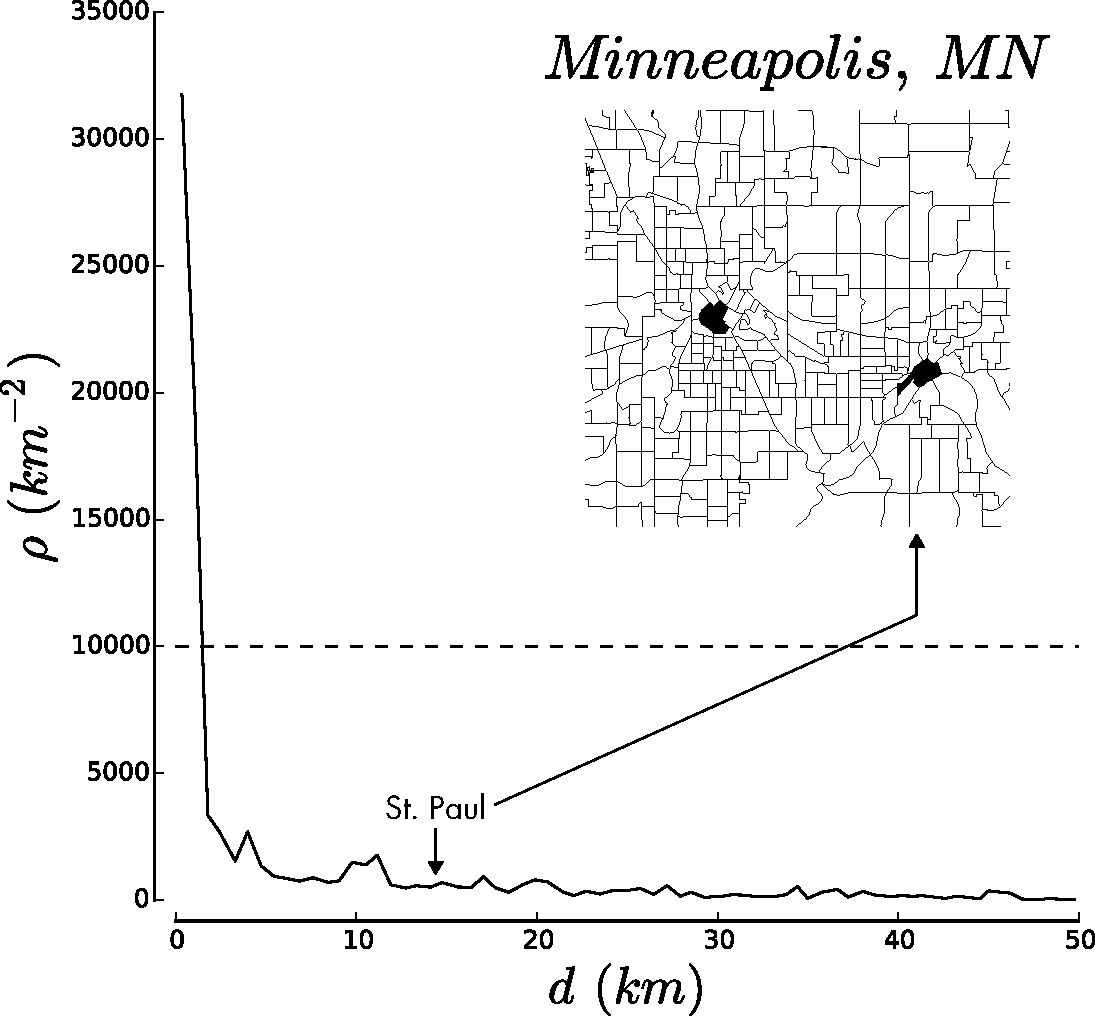
\includegraphics[width=\textwidth]{./gfx/chapter-monocentric/distance_center_minneapolis.pdf}
    \caption{(Left) Employment density as a function of distance to the center for the
    Metropolitan Area of Minneapolis-St. Paul in 2000. The center is defined here as the
    tract with the highest employment density. The curve exhibits a very sharp
    decay, giving the illusion of a monocentric structure. (Right) The census tracts
    of Minneapolis-St. Paul in 2000. In black, the census tracts where the
    employment density reaches values above $10,000\,\text{km}^{-2}$. The two tracts
    coincide with the historical centers of the Twin Cities, and are distant from
    $x\,\text{km}$. This fragmented structure cannot be infered from the density
    profile on the left.
    \label{fig:distance_center_Minneapolis}}
\end{figure}

The problem with the traditional models of cities in two pictures: the
(polycentric) reality and the AMM model.

\cite{Harris:1945} multiple centers, multi-nucleated cities\\

The Alonso-Muth-Mills model might well be the reason for the long-lasting influence of
the monocentric model (a nice exposition of the model can be found
in~\cite{Fujita:1989}). In 1964, Alonso introduced the bid-rent curve as a
function of the distance to the city center~\cite{Alonso:1964}. The simplifying hypothesis of
\emph{monocentricity} naturally followed, the assumption that all firms in a
city are concentrated in a single, fixed-size part of the city, the central business
district. We should not underestimate how this model influenced many people's
perception of what a city is. In the US, the name of Central Business District
is casually used as a way to designate the principle activity center in a city.
Many, if not most, measures of the spatial variation of quantities inside cities
actually use the notion of `distance to the city center'. This only makes sense,
however, under the assumption of monocentricity. Most of the
literature has not departed from the monocentric assumption---sometimes without
being aware of it! In the defense of these authors however, there is a clear
lack of appropriate tools to study spatial profiles.


\cite{Mills:1972} is a monograph discussing the causes of decentralisation and
suburbanisation. [could not read]

\cite{Kemper:1974} explores data trying to fit a negative exponential function
to industry and employment density. It does not work so well.

\cite{Odland:1978} explores the possibility of polycentric cities on a
theoretical basis. [could not read]

\cite{Griffith:1981} tool to evaluate the polycentricity of a pattern.[could not
read]

Treatment of the polycentric city in the urban economics literature starts
with~\cite{Fujita:1982}.

\cite{Dokmeci:1994} shows that Istanbul's employment is spread across several
centers. Although there is still a lack of strong quantitative evidence, the
idea is gaining ground.

\cite{Garreau:1991} Edge cities.

\cite{Gordon:1996} Beyond polycentricity: the dispersed city.

\section{Reasons invoked for the polycentric transition}
\label{sec:reasons_invoked_for_the_polycentric_transition}

We exlude the cases where polycentrism finds its origin in the fusion of two
Metropolises (Copenhagen-Malm\"o, Twin Cities, Ruhr) or through the
incorporation of satellite municipalities.\\


\cite{McMillen:2003} suggests congestion might be the reason for polycentrism.



\section{How to measure polycentrity}
\label{sec:how_to_measure_polycentrity}

\cite{Tsai:2005} is a classic on Urban Form, along with~\cite{LeNechet:2015} and
\cite{Schwarz:2010}.

\cite{McDonald:1987} proposes the first empirical method to identify employment
subcenters.

\cite{Giuliano:1991} uses an arbitrary threshold to determine the centers.

\cite{Anas:1998} Critices the method of Giuliano, has a cool picture of
Los-Angeles spreading and deals with urban structure.

\cite{Bertaud:2001} is very interesting on urban form in general, and proposes
an index, the eccentricity, to measure the distance of the center of gravity to
the geographical CBD.


\cite{McMillen:2001} proposes a non-parametric method to find the subcenters.

\cite{McMillen:2003} proposes a pretty good literature review in introduction on
the identification of employment subcenters, and proposes congestion as a reason
for the polycentric transition.


\cite{Griffith:2007} is yet another reference on spatial regression.\\

\cite{Redfearn:2007} Proposes interesting visualisations and a parametric method
to determinate the number of centers.\\

Have a look at what~\cite{Berroir:2008} do!


\cite{LeNechet:2010} introduces the acentrism index (also explained
in~\cite{LeNechet:2015}.\\

\cite{Pereira:2013} proposes an Urban Centrality Index that varies continuously
between a monocentric configuration and an extreme decentralized situation.

\cite{Louf:2013_polycentric} Proposes to use a property of the rank plot of the
employment density, exponential decrease.

\cite{Louail:2014} proposes a generalisation of the previous method based on the
Lorenz curve.

I propose a generalisation, based on the same hypothesis but that is more robust
than the computation of the tangent at the origin.

Justify the term `polycentric transition'. When the population increases, it is
clear that the number of centers increases as well. Therefore, it seems that, as
they grow and expand, urban systems develop a more and more polycentric form.
